\tikzstyle{input} = [coordinate]
\tikzstyle{output} = [coordinate]

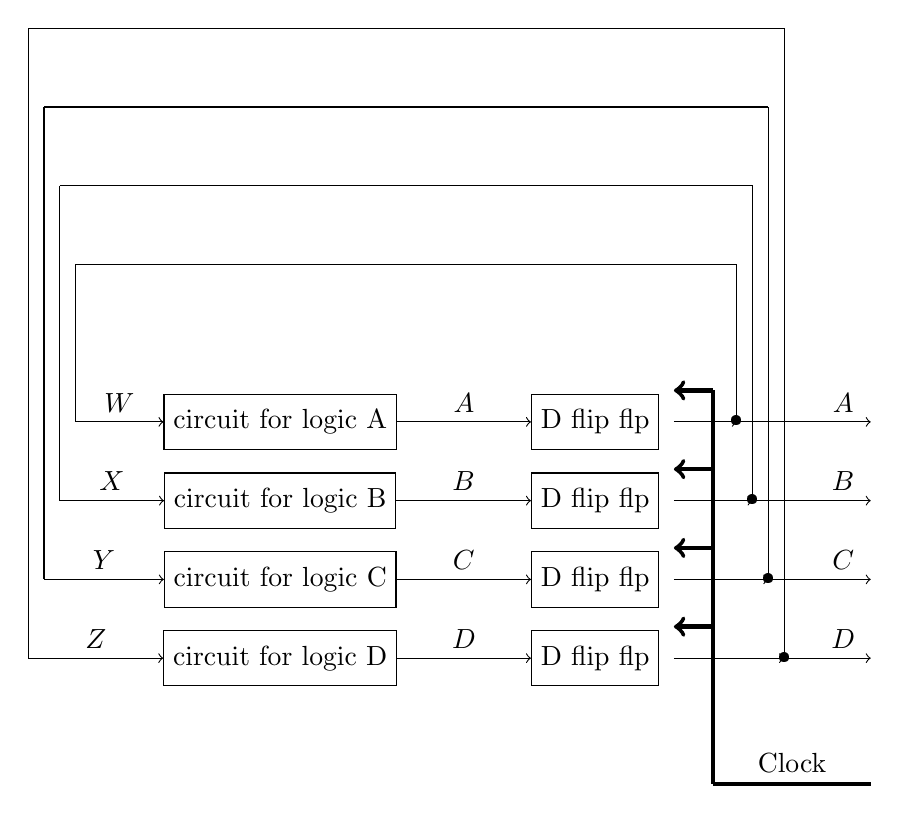
\begin{tikzpicture}
\tikzstyle{block} = [draw,minimum size=2em]
\node at (0,-1) (input 1) {$$};
\node at (0,-2) (input 2) {$$};
\node at (0,-3) (input 3) {$$};
\node at (0,-4) (input 4) {$$};
\node[block] at (2,-1) (block1) {circuit for logic A};
\node[block] at (2,-2) (block2) {circuit for logic B};
\node[block] at (2,-3) (block3) {circuit for logic C};
\node[block] at (2,-4) (block4) {circuit for logic D};
\node[block] at (6,-1) (block5) {D flip flp};
\node[block] at (6,-2) (block6) {D flip flp};
\node[block] at (6,-3) (block7) {D flip flp}; 
\node[block] at (6,-4) (block8)  {D flip flp};
\draw [->] (block1) -- node[above,name=A] {$A$} (block5);
\draw [->] (block2) -- node[above,name=A] {$B$} (block6);
\draw [->] (block3) -- node[above,name=A] {$C$} (block7);
\draw [->] (block4) -- node[above,name=A] {$D$} (block8);
\node [output, right of=block5] (output 1) {};
\node [output, right of=block6] (output 2) {};
\node [output, right of=block7] (output 3) {};
\node [output, right of=block8] (output 4) {};
\draw[->] (output 1) -- (7.8,-1);
\draw[->] (output 2) -- (8,-2);
\draw[->] (output 3) -- (8.2,-3);
\draw[->] (output 4) -- (8.4,-4);
\draw (7.8,-1) -- (7.8,1);
\draw (8,-2) -- (8,2);
\draw (8.2,-3) -- (8.2,3);
\draw (8.4,-4) -- (8.4,4);
\foreach \Point in {(7.8,-1), (8,-2), (8.2,-3), (8.4,-4)}{
    \node at \Point {\textbullet};
}
\draw (7.8,1) -- (-0.6,1);
\draw (8,2) -- (-0.8,2);
\draw (8.2,3) -- (-1,3);
\draw (8.4,4) -- (-1.2,4);
\draw (-0.6,1) -- (-0.6,-1);
\draw (-0.8,2) -- (-0.8,-2);
\draw (-1,3) -- (-1,-3);
\draw (-1.2,4) -- (-1.2,-4);
\draw[ultra thick,->](7.5,-0.6) -- (7,-0.6);
\draw[ultra thick](7.5,-0.6) -- (7.5,-1.6);
\draw[ultra thick,->](7.5,-1.6) -- (7,-1.6);
\draw[ultra thick](7.5,-1.6) -- (7.5,-2.6);
\draw[ultra thick,->](7.5,-2.6) -- (7,-2.6);
\draw[ultra thick](7.5,-2.6) -- (7.5,-3.6);
\draw[ultra thick,->](7.5,-3.6) -- (7,-3.6);
\draw[ultra thick](7.5,-3.6) -- (7.5,-5.6);
\draw [ultra thick] (7.5,-5.6) -- node[above] {Clock} (9.5,-5.6);
\draw (7.8,-1) -- node[above] { $$} (8.8,-1);
\draw (8,-2) -- node[above] { $$} (8.8,-2);
\draw (8.2,-3) -- node[above] { $$} (8.8,-3);
\draw (8.4,-4) -- node[above] { $$} (8.8,-4);
\draw [->] (8.8,-1) -- node[above] { $A$} (9.5,-1);
\draw [->] (8.8,-2) -- node[above] { $B$} (9.5,-2);
\draw [->] (8.8,-3) -- node[above] { $C$} (9.5,-3);
\draw [->] (8.8,-4) -- node[above] { $D$} (9.5,-4);
\draw [->] (-0.6,-1) -- node[above] {$W$} (block1);
\draw [->] (-0.8,-2) -- node[above] {$X$} (block2);
\draw [->] (-1,-3) -- node[above] {$Y$} (block3);
\draw [->] (-1.2,-4) -- node[above] {$Z$} (block4);
\end{tikzpicture}
